\begin{minipage}{\linewidth}
\begin{table}[H]
    \centering
    \caption{AC-AC Voltage Transformator Data }
    \label{tab:voltage transformator }
    \small
    \begin{tabular*}{\linewidth}{@{\extracolsep{\fill}}ccc}
    \textbf{V (input) (V)} &\textbf{I (mA)} &\textbf{V(output) (mV)} \\\midrule
    10 &0.59 &3.6 \\
    20 &1.15 &8.6 \\
    30 &1.7 &12.8 \\
    40 &2.25 &16.9 \\
    50 &2.8 &21.2 \\
    60 &3.4 &25.3 \\
    70 &3.96 &29.6 \\
    80 &4.52 &33.6 \\
    90 &5 &38 \\
    100 &5.67 &42.2 \\
    110 &6.21 &46.4 \\
    120 &6.77 &51 \\
    130 &7.38 &55.2 \\
    140 &7.9 &59.1 \\
    \bottomrule
    \end{tabular*}
\end{table}
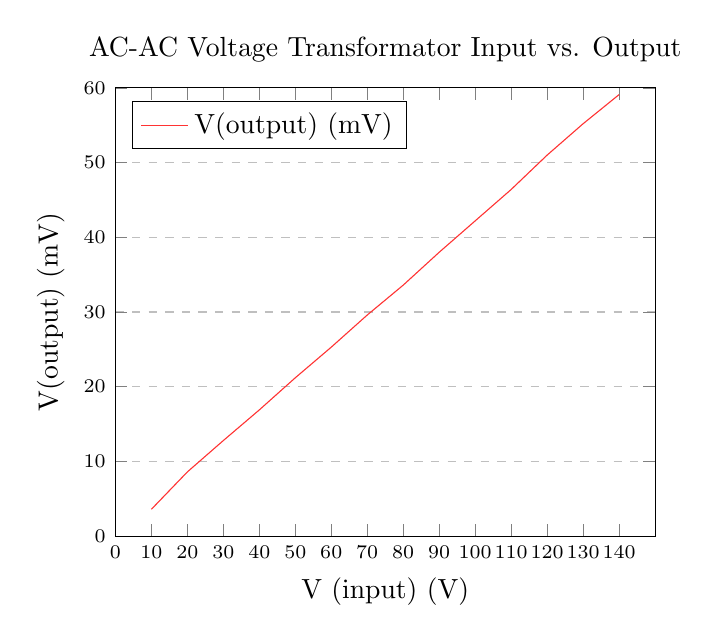
\begin{tikzpicture}
    \begin{axis}[
    title={AC-AC Voltage Transformator Input vs. Output},
    ticklabel style={font=\scriptsize},
    xlabel={V (input) (V)},
    ylabel={V(output) (mV)},
    xmin=0, xmax=150,
    ymin=0, ymax=60,
    xtick={0,10,20,30,40,50,60,70,80,90,100,110,120,130,140},
    ytick={0,10,20,30,40,50,60},
    legend pos=north west,
    ymajorgrids=true,
    grid style=dashed,
    xmajorgrids=false
]
    \addplot[
        color=red!80,
        mark=circle,
    ]
    coordinates {
        (10,3.6)(20,8.6)(30,12.8)(40,16.9)(50,21.2)(60,25.3)(70,29.6)(80,33.6)(90,38)(100,42.2)(110,46.4)(120,51)(130,55.2)(140,59.1)
    };
    \addlegendentry{V(output) (mV)}
    \label{fig:V in-out}
    \end{axis}
\end{tikzpicture}
\end{minipage}